%\chapter{Dispositif expérimental : des atomes de Rydberg sur puce}
%\label{chapter:setup_ryd}
%
%\section{Excitation et détection d'atomes de Rydberg}
%	\subsection*{Schémas d'excitation}
%		\noindent schéma laser : schéma de niveaux (60s ou 50d) et schéma optique		
%	\subsection*{Schémas de détection}
%		\noindent state selective ionization
%		\noindent signaux d'ionisation et toutes les subtilités
%		
%\section{Problème des champs électriques près d'une puce}
%	\subsection*{L'élargissement Stark inhomogène}
%		\noindent raies de plusieurs dizaines de MHz de large, drift
%	\subsection*{Recouvrir la puce de rubidium}
%		\noindent dispositif dispensers et raies fines
%	\subsection*{Contrôle du champ électrique}
%		\noindent Lhomond et CdF, électronique de contrôle \\
%		\noindent électrodes RF pour la circularisation (Simion ?) 
%		
%\section{Spectroscopie microonde}
%	\noindent mention rapide des domaines de transition entre les niveaux de Rydberg
%	
\section{Excitation et détection d'atomes de Rydberg près d'une puce}
intro de la section :\\
??

	\subsection{L'excitation à deux photons des atomes de Rydberg}

\noindent Les atomes de rubidium piégés dans un nuage près de la puce sont excités vers les niveaux de Rydberg par une transition laser à deux photons désaccordée par rapport au niveau intermédiaire.
Dans nos recherches, deux niveaux de Rydberg différents ont été excités par laser à partir de l'état fondamental 5S$_{1/2}$ : le niveau 60S$_{1/2}$ et le niveau 50D$_{3/2}$.
Nous décrivons ici l'excitation d'un nuage d'atomes de Rydberg au sein d'un nuage froid dans le piège magnétique, en négligeant les interactions entre atomes de Rydberg et en nous concentrant sur le niveau $\mathrm{60S_{1/2}}$.

La transition du niveau fondamental au niveau de Rydberg est faite par l'absorption d'un photon rouge à $\lambda = \SI{780}{\nano\meter}$, désaccordé de $\delta=+\SI{540}{\MHz}$ par rapport à la transition $\mathrm{5S_{1/2},F=2 \rightarrow 5P_{3/2},F'=3}$, et d'un photon bleu à $\lambda = \SI{480}{\nano\meter}$, accordé pour satisfaire la condition de résonance vers le niveau choisi.
La figure \eqref{fig:2photons} représente le schéma de niveaux de l'excitation du niveau $\mathrm{60S_{1/2}}$.
Les deux faisceaux d'excitation sont superposés et se propagent selon la direction $+x$. Leurs polarisations sont définies par rapport à l'axe de quantification des niveaux atomiques, déterminé par le champ magnétique de biais $B_x$ dans le fond du piège.
La figure \eqref{fig:lasers_excit} représente la géométrie des faisceaux laser d'excitation.
Dans cette configuration, seul le sous-niveau $m_j=+1/2$ du niveau 60S est excité.
%
\begin{figure}[!h]
\centering
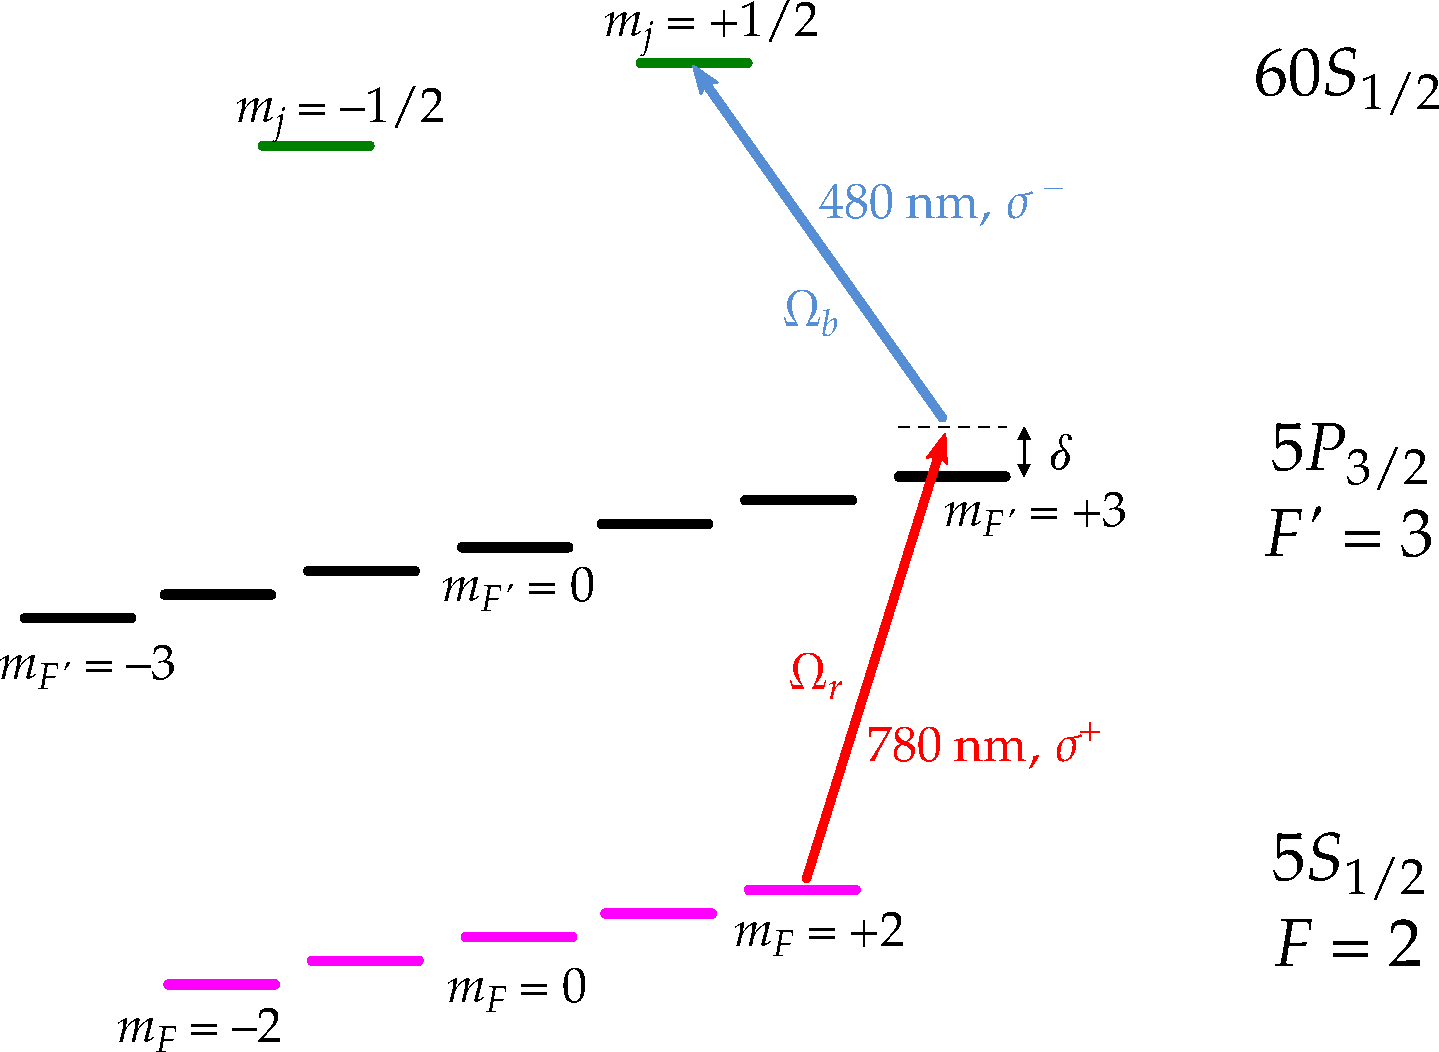
\includegraphics[width=.8\linewidth]{figures/2photons}
\caption[Excitation du niveau 60S]{Schéma de l'excitation laser du niveau 60S, à partir d'atomes de \Rb{87} dans le niveau fondamental dans le piège magnétique.
La polarisation de chaque laser est indiquée.
$\Omega_r$ et $\Omega_b$ sont les fréquences de Rabi des transitions à \num{780} et \SI{480}{\nano\meter} respectivement.
$\delta=\SI{540}{\MHz}$ est le désaccord par rapport au niveau intermédiaire.
}
\label{fig:2photons}
\end{figure}

Le faisceau rouge a typiquement un col de $\SI{150}{\um}$ et une puissance de $\SI{50}{\micro\watt}$ au niveau des atomes.
Le laser rouge est désaccordé de $\delta=\SI{540}{\MHz}$ par rapport à la transition $ \ket{\mathrm{5S_{1/2},F=2,m_F=+2}} \rightarrow \ket{\mathrm{5P_{3/2},F'=3,m_F'=+3}}$, dont le moment de transition dipolaire vaut $\SI{2.98931 (62)} ea_0$ \cite{DATA_STECKRB87}.
D'après les caractéristiques du faisceau, la fréquence de Rabi correspondant à cette transition est de l'ordre de $\Omega_r \simeq 2\pi\times \SI{40}{\MHz}$.
Le taux d'émission spontanée de photons rouge par le niveau intermédiaire, de durée de vie $\Gamma^{-1} \simeq \SI{26}{\ns}$, est donné par
\begin{equation}
\label{eq:scattering_5P3/2}
\Gamma_{sp} = \frac{1}{2} \frac{\Omega_r^2 \Gamma}{\delta^2 + \Omega_r^2 + \Gamma^2}
\simeq \frac{\Omega_r^2}{2\delta^2} \Gamma,
\end{equation}
où $\Gamma = 2\pi \times 6.065 MHz$ est la largeur naturelle du niveau $\mathrm{5P_{3/2}}$.
La dernière égalité est vérifiée dans l'approximation $\delta^2 \gg \Omega_r^2, \Gamma^2$, qui est ici valide.
Avec nos valeurs d'intensité et de désaccord du laser, on obtient $\Gamma_{sp} \simeq \num{2.5e-3} \Gamma = 2\pi\times \SI{0.657}{\MHz}$, ce qui correspond à l'émission d'un photon  toutes les $\Gamma_{sp}^{-1} = \SI{0.24}{\us}$.
Or lorsqu'un atome absorbe et ré-émet un tel photon, il gagne une énergie moyenne
$\Delta E = p^2/(2m_{Rb87}) = h^2/(2m_{Rb87} \lambda^2) = \SI{180}{\nano\kelvin} / \kb$.
Le piège est ainsi chauffé par le laser rouge d'excitation, ce qui limite à la fois la puissance que l'on peut envoyer sur le nuage, et le nombre d'impulsions laser d'exciation que l'on peut faire subir à un même nuage sans l'altérer.

Le faisceau bleu a typiquement un col de $\SI{22}{\um}$ et une puissance estimée à $\SI{4}{\milli\watt}$ au niveau des atomes.
Le moment dipolaire de la transition $ \ket{\mathrm{5P_{3/2},F'=3,m_F'=+3}} \rightarrow \ket{\mathrm{60S_{1/2},m_j=+1/2}}$ est cependant bien plus faible que le précédent, et vaut $\SI{9.9e-3} ea_0$
\footnote{Nous rappelons ici que, comme nous l'avons mentionné en \ref{sec:alkalRydberg}, le bon nombre quantique magnétique pour les niveaux de Rydberg est $m_j$ et non pas $m_F$.}.
La fréquence de Rabi pour cette transition est alors de $\Omega_b = 2\pi\times \SI{8}{\MHz}$.
Les fréquences de Rabi des deux trasitions satisfont l'approximation $\Omega_{r,b} \ll \delta$, ce qui nous permet de négliger l'occupation du niveau intermédiaire, et donc de l'éliminer adiabatiquement \cite{TXT_ASPECTFABRE_QUANTOPT}.
Le système à trois niveaux se ramène alors à un système effectif à deux niveaux, couplés par une fréquence de Rabi
\begin{equation}
\label{eq:Rabi_2photons}
\Omega = \frac{\Omega_r \Omega_b}{\delta}.
\end{equation}
Avec nos paramètres, on obtient une fréquence de Rabi $\Omega = 2\pi \times \SI{296}{\kHz}$ pour la transition $\ket{\mathrm{5S_{1/2},F=2,m_F=+2}} \rightarrow \ket{\mathrm{60S_{1/2},m_j=+1/2}}$.
Ce paramètre peut être varié simplement en ajustant la puissance du laser rouge ou la puissance du laser bleu.

%
\begin{figure}[!h]
\centering
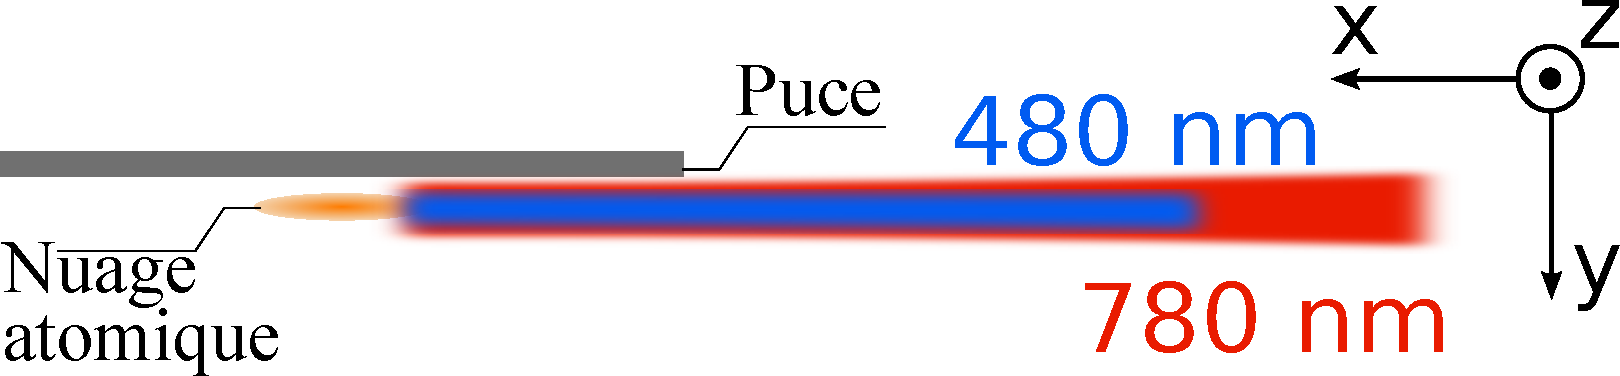
\includegraphics[width=.8\linewidth]{figures/lasers_excit}
\caption[Faisceaux laser pour l'excitation des Rydberg]{Schéma représentant la géométrie des faisceaux laser d'excitation.
}
\label{fig:lasers_excit}
\end{figure}

		
	\subsection{La détection par ionisation des atomes de Rydberg}
\noindent L'électron de valence d'un atome de Rydberg alcalin est très proche du seuil d'ionisation.
Il est donc très facile de l'arracher au noyau en appliquant un champ électrique.
Nous exploitons cette caractéristique pour détecter les atomes de Rydberg par ionisation en champ électrique :
une fois l'atome ionisé, le c\oe ur atomique est accéléré par des électrodes vers un détecteur à avalanche (Channeltron).


%
\begin{figure}[h]
\centering
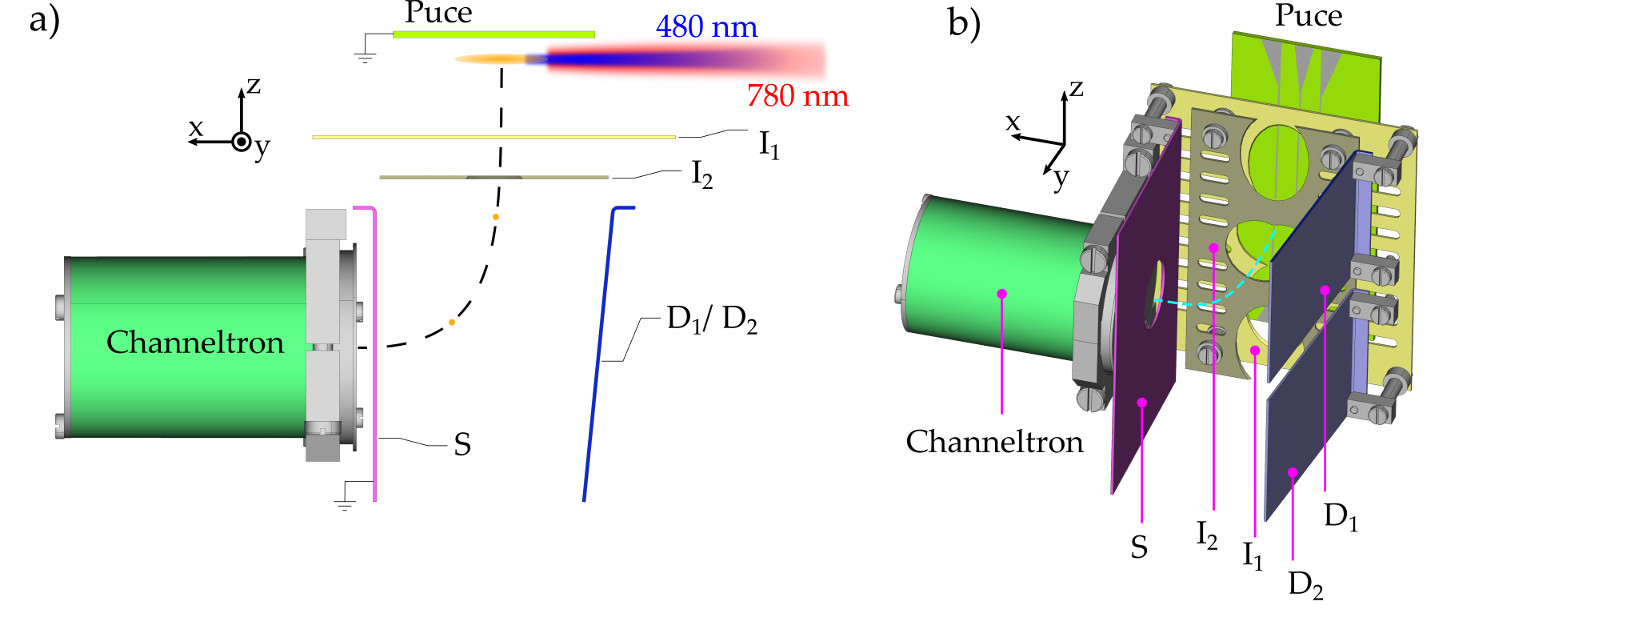
\includegraphics[width=\linewidth]{figures/schema_detect}
\caption[Système de détection des atomes de Rydberg]{Schéma représentant le système de détection des atomes de Rydberg.
\textbf{a)} vu de dessus et \textbf{b)} en projection axonométrique.
Après excitation, les atomes de Rydberg sont ionisés par les élctrodes $I_1$ et $I_2$.
Les ions ainsi créés et accélérés sont défléchis par les électrodes $D_1$ et $D_2$, en direction du détecteur Channeltron.
L'électrode $S$ est mise à la masse et sert à écranter la tension présente à l'entrée du Channeltron.
La trajectoire des ions est indiquée en lignes pointillées et les faisceaux lasers d'excitation sont représentés en \textbf{a)}.
}
\label{fig:schema_detect}
\end{figure}
%
La figure \eqref{fig:schema_detect} présente un schéma détaillé du système de détection par ionisation.
Au moment de la détection, une tension négative est appliquée sur les électrodes d'ionisation $I_1$ et $I_2$.
La tension sur ces électrodes crée un champ électrique au niveau des atomes, la puce étant mise à la masse.
Ce champ électrique ionise les atomes de Rydberg et accélère les ions positifs ainsi créés.
Ces ions sont ensuite défléchis en direction du Channeltron par les électrodes $D_1$ et $D_2$, chargées en permanence à une tension $V_{defl} = +\SI{150}{\V}$.
Une grille placée à l'entrée du Channeltron est alimentée par une tension de $\SI{-3000}{\V}$.
Une électrode trouée mise à la masse est placée devant cette grille afin d'écranter les $\SI{-3000}{\V}$ pour la région de piégeage des atomes.
Lorsque les ions arrivent dans le Channeltron, celui-ci génère par avalanche un signal électronique qui est envoyer vers un amplificateur et un discriminateur permettant de décompter les ions détectés.
Le Channeltron est isolé thermiquement et chauffé à une température de $\SI{42}{\K}$ afin d'augmenter son efficacité.

\subsubsection*{Sélectivité de niveau de la détection par ionisation}
\noindent Chaque atome de Rydberg présente une énergie différente, telle que discutée en \ref{sec:alkalRydberg}.
Cela signifie qu'ils sont tous à une distance différente du seuil d'ionisation, et \textit{in fine} que chaque niveau de Rydberg sera ionisé pour une valeur de champ électrique spécifique.
L'on peut ainsi appliquer une rampe de tension sur les électrodes d'ionisation, afin que chaque niveau de Rydberg soit ionisé à un instant différent.
Alors, les ions correspondants arriveront à des instants différents au Channeltron et pourront être distingués.
La figure \eqref{fig:arrTimes6057} montre un signal de détection sélective des niveaux de Rydberg $\mathrm{60S_{1/2}}$ et $\mathrm{57S_{1/2}}$.
La rampe de tension et les fenêtres temporelles de détection sont optimisées afin de distinguer au mieux les différents niveaux de Rydberg détectés.
L'efficacité de détection de notre dispositif a été mesurée à $\SI{90}{} \pm \SI{10}{\percent}$.
%
\begin{figure}[h]
\centering
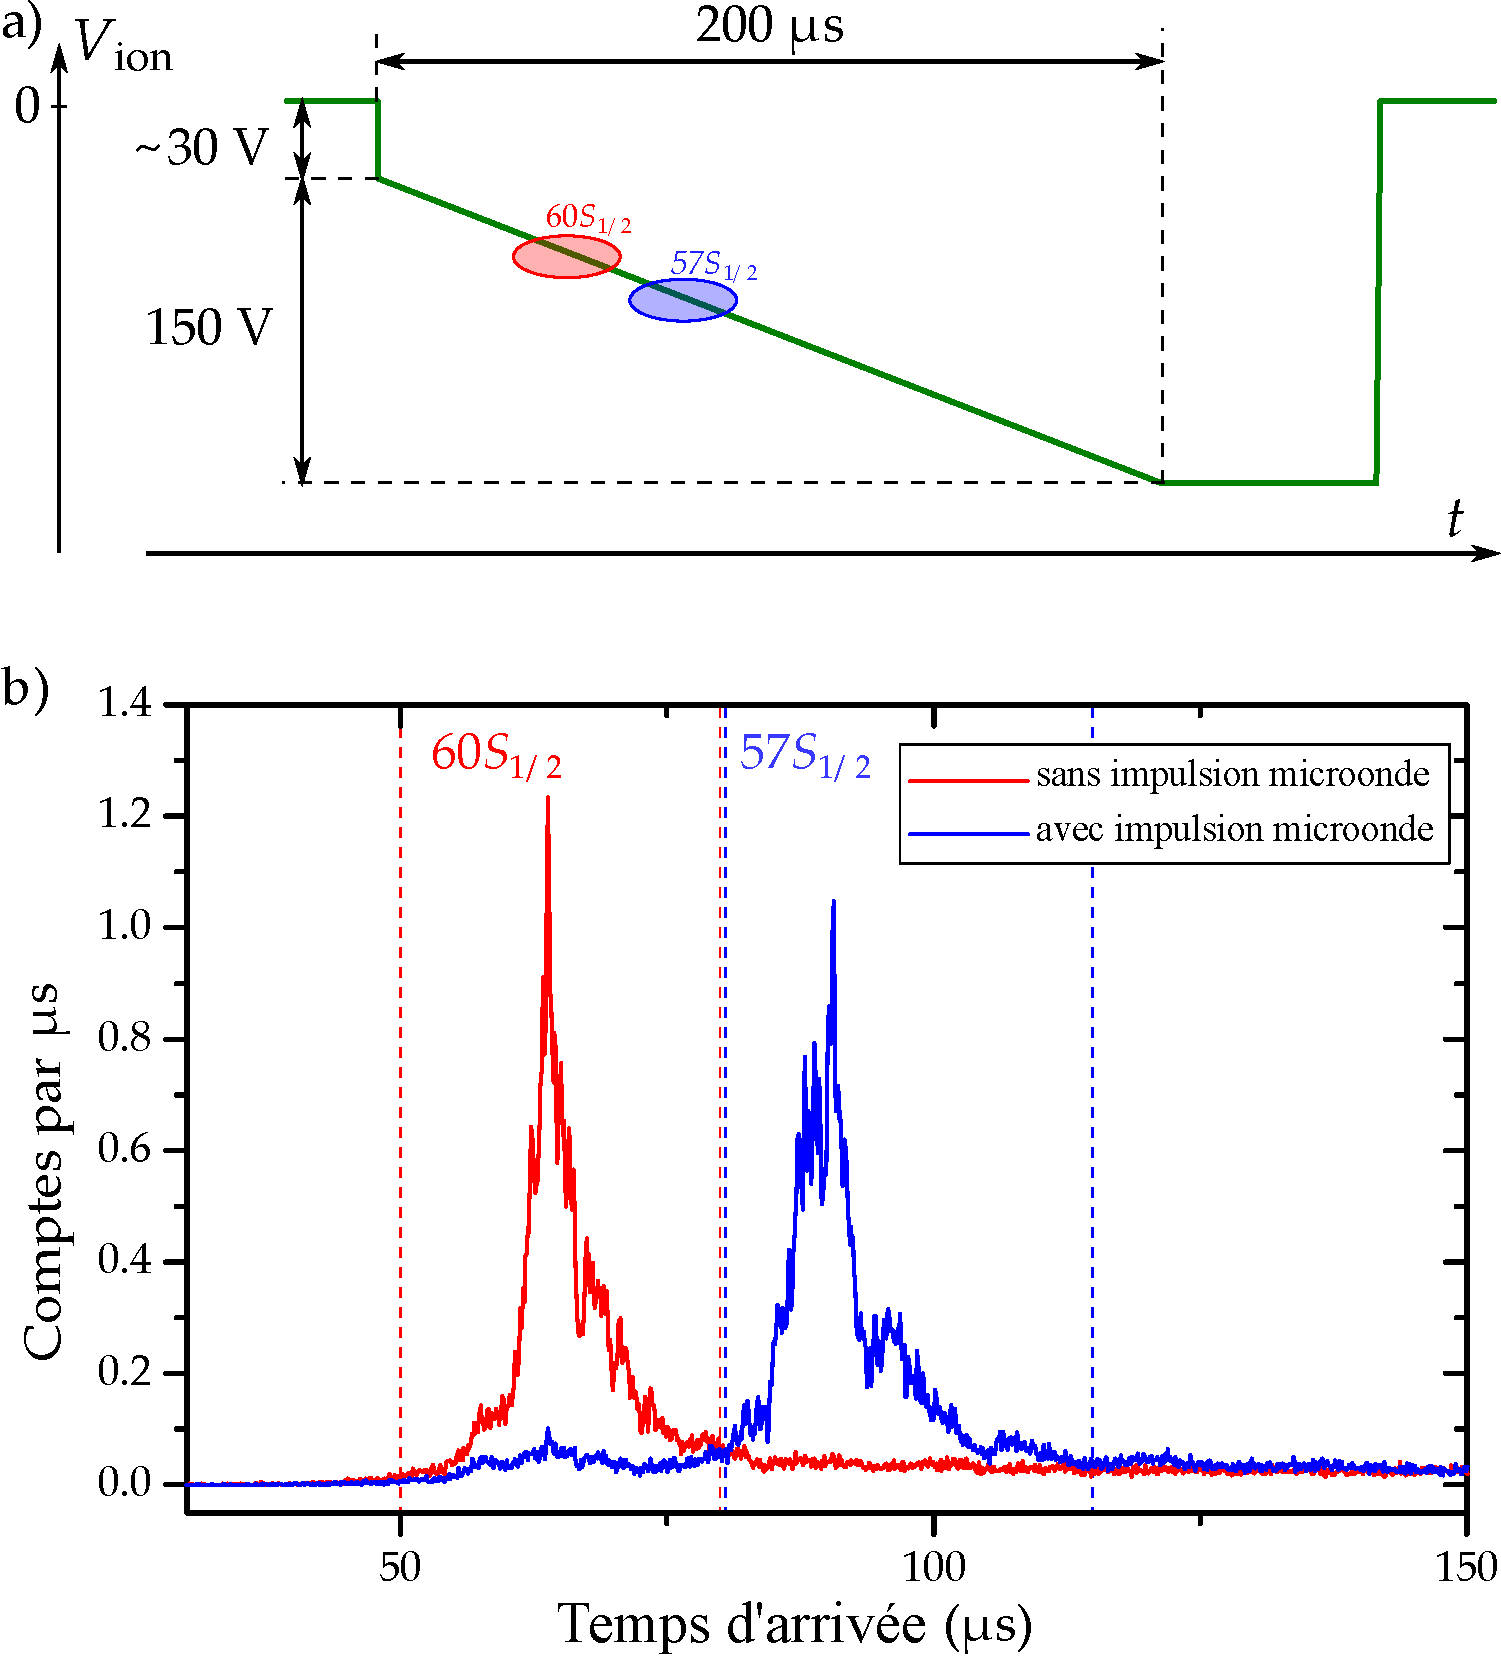
\includegraphics[width=.7\linewidth]{figures/arrTimes6057}
\caption[Détection sélective des niveaux $\mathrm{60S_{1/2}}$ et $\mathrm{57S_{1/2}}$]{
Détection sélective des atomes de Rydberg.
\textbf{a)} une rampe de tension $V_{ion}$ typique appliquée sur les électrodes d'ionisation.
Les seuils d'ionisation des niveaux $\mathrm{60S_{1/2}}$ et $\mathrm{57S_{1/2}}$ sont indiqués en rouge et bleu respectivement.
\textbf{b)} Temps d'arrivée des ions correspondants. Des fenêtres temporelles de détection, représentées en pointillés, sont définies pour compter sélectivement les atomes dans les niveaux $\mathrm{60S_{1/2}}$ et $\mathrm{57S_{1/2}}$.
Les atomes sont préparés dans l'état $\mathrm{60S_{1/2}}$ et le niveau $\mathrm{57S_{1/2}}$ est peuplé par une impulsion $\pi$ de la transition microonde adéquate.
Les échelles de temps sont différentes en \textbf{a)} et \textbf{b)}.
}
\label{fig:arrTimes6057}
\end{figure}
%


%EJECTE : note sur l'ionisation diabatique vs adiabatique. 
		
	\subsection{Les champs électriques parasites, défi des atomes de Rydberg sur puce}\label{subsec:flashRb}
	%problème des champs électriques et flash de Rb}
\noindent Comme nous l'avons dit au chapitre \ref{chapter:Rydberg}, les atomes de Rydberg sont des objets extrêmement sensibles au champ électromagnétique.
Or, dans notre expérience, nous souhaitons exciter et manipuler des atomes de Rydberg à proximité immédiate d'une surface, la puce à atomes.
Les bruits électriques étant inévitables près d'une surface, la présence de la puce va rendre difficile l'excitation et la manipulation des atomes de Rydberg.

\subsubsection*{Premiers spectres}
\noindent Ce problème est très clair sur les premiers spectres que nous avons fait de la transition $\ket{\mathrm{5S_{1/2}}} \rightarrow \ket{\mathrm{60S_{1/2}}}$, présentés en figure \eqref{fig:vieilles_raies}.

\begin{figure}[]
\centering
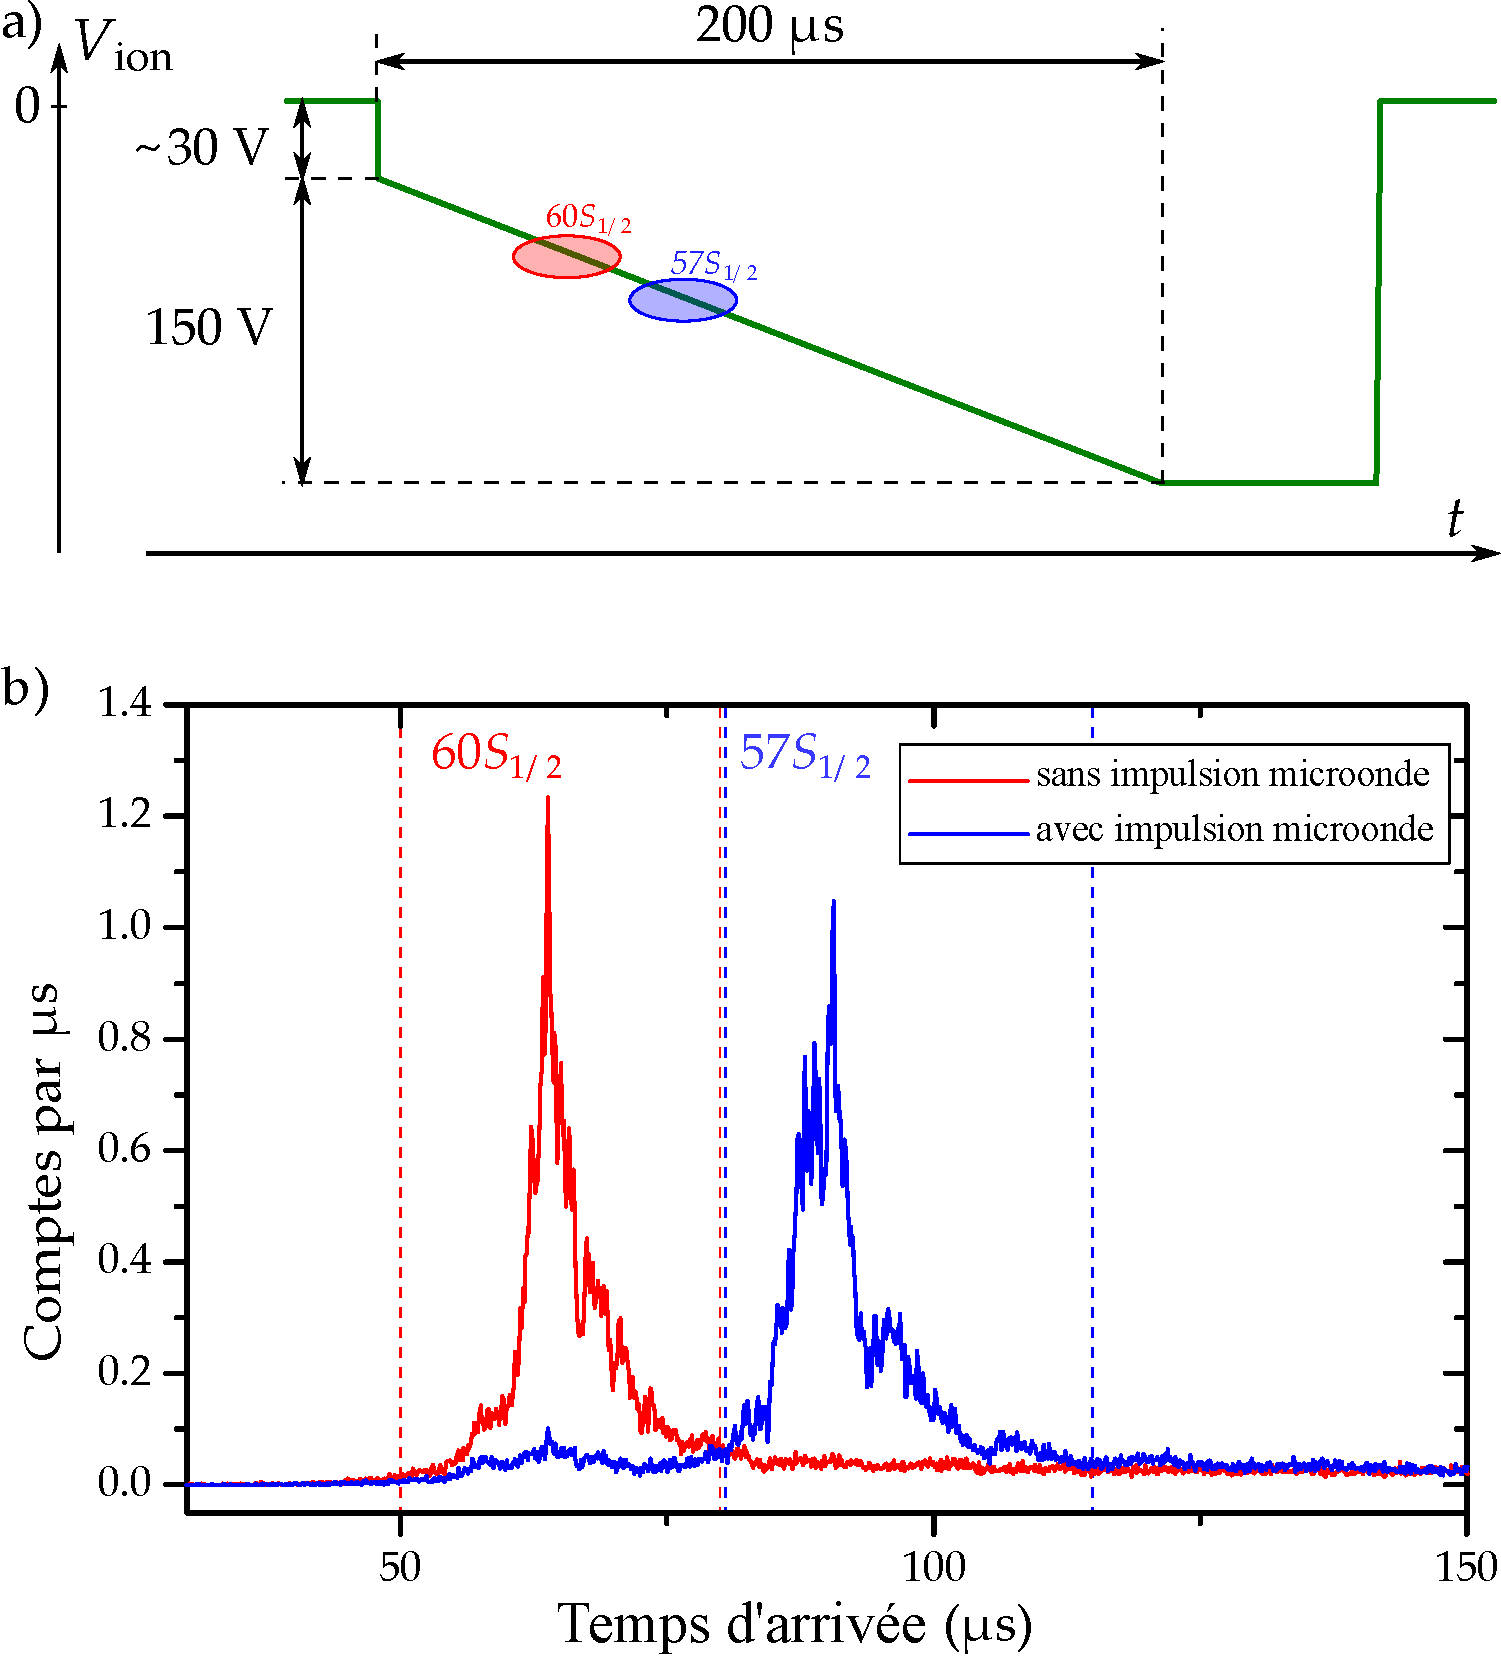
\includegraphics[width=\linewidth]{figures/arrTimes6057}
\caption[Spectres d'excitation laser 5S-60S avant le dépôt de rubidium sur la puce]{
Deux spectres laser de la transition $5\mathrm{S}\rightarrow60\mathrm{S}$, avant correction des inhomogénéités et de la dérive du champ électrique.
Leurs largeurs sont de $\SI{30}{\MHz}$ et $\SI{40}{\MHz}$ respectivement, et ils sont décalés en fréquence de $\SI{12}{\MHz}$ l'un par rapport à l'autre.}
\end{figure}

	\newpage
	on travaille près d'une puce qui est une surface, et avec des objets ultra-sensibles -> ça peut créer des problèmes ! \\
		\noindent vieilles raies larges et moches : expliquer par l'effet Stark quadratique et l'élargiseement inhomogène. \\
		\noindent potentiel de contact et flash de Rb : dessins et schéma + dispensers et leur emplacement et boîte de protection \\
		\noindent c'est magiques, ça nous donne de belles raies fines !
		
	\subsection{compensation et contrôle des champs}
	c'est bien d'avoir' ces raies fines mais on veut contrôler le champ électrique le mieux possible
		\noindent électrode Vcomp et schéma de contrôle mixte excitation/détection. Le contrôle du champ sur $Oy$ c'est bien, ça permet de faire plein de trucs, mais il reste des gradients (au moins).\\
		
		\noindent si on veut faire encore mieux, il faut contrôler les champs selon $Ox$ et $Oy$ $\rightarrow$ électrodes RF :
		\\ schéma d'installation des électrodes
		\\ SIMION pour vérifier que ça permet de créer des champs y compris très près de la puce
		\\ en plus, ça servira de source de RF polarisée !!
		
	\subsection{manipulation et observation des Rydbergs}
\noindent C'est bien de détecter des Rydberg, mais il faut aussi pouvoir les manipuler et les caractériser.
Pour ça, on a un outil fabuleux : la spectroscopie microonde vers les niveaux voisins ! \\
schéma de niveaux ? schéma de dispositif ? \\
on peut mentionner ici qu'avec ça on a pu calibrer les champs électriques résiduels, et faire un qubit $60s-61s$ qui vit très longtemps.

\section*{Conclusion}
On a un dispositif lourd et complexe mais qui permet de faire beaucoup de belles choses avec des Rydbergs ultra-froids.